\documentclass[a4paper,12pt]{article} 
\usepackage[top=15mm,left=12.5mm, right=12.5mm]{geometry}

% Рисунки
\usepackage{graphicx}
\usepackage{wrapfig}

%  Русский язык
\usepackage[T2A]{fontenc}			% кодировка
\usepackage[utf8]{inputenc}			% кодировка исходного текста
\usepackage[english,russian]{babel}	% локализация и переносы

% Математика
\usepackage{amsmath,amsfonts,amssymb,amsthm,mathtools} 
\usepackage{mathrsfs}

\usepackage{wasysym}

\begin{document} % начало документа

Logovsky Yan, 711 group\\
March 2019

\begin{center}
Model of rotating body
\end{center}

In this project I have inplemented simulation of solid body rotation.\\
\begin{enumerate}
\item simulator, written on C language, uses runge kutta method to compute parameters of model at the time, which is gradually changes.
\item simulator dumps those parameters into data files.
\item jupyter-notebook reads data from those files and draws a plot for each stage of our model and save this plot as an image.
\item unix application ffmpeg makes a video from frames.
\end{enumerate}

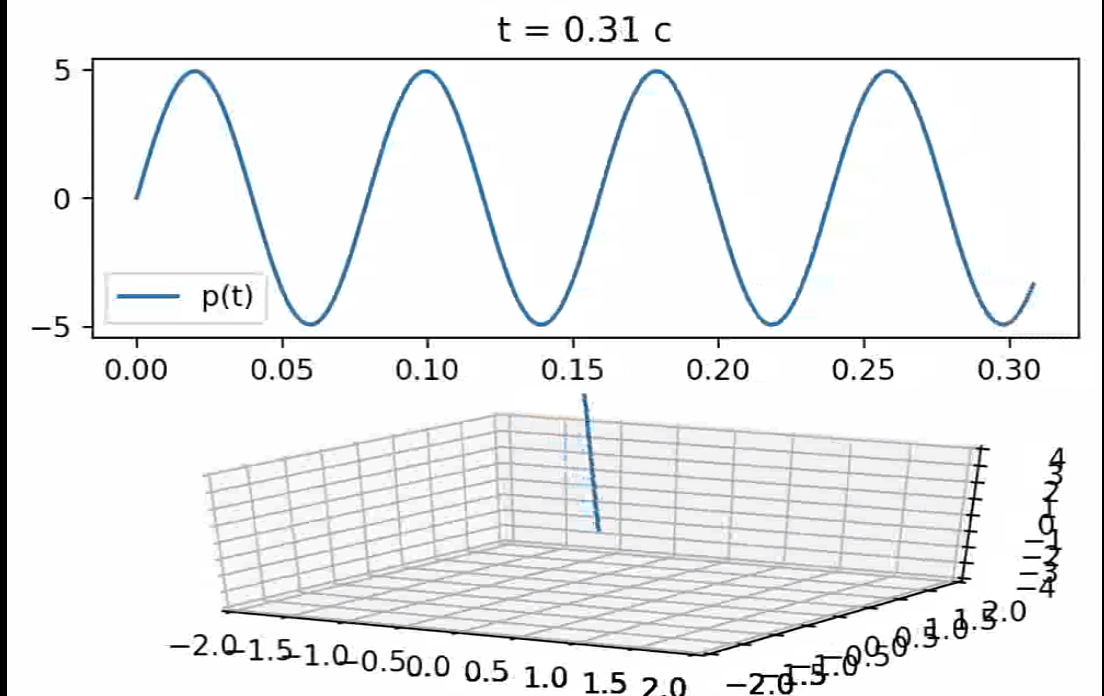
\includegraphics[width = 0.5 \textwidth]{euler_case_regular}
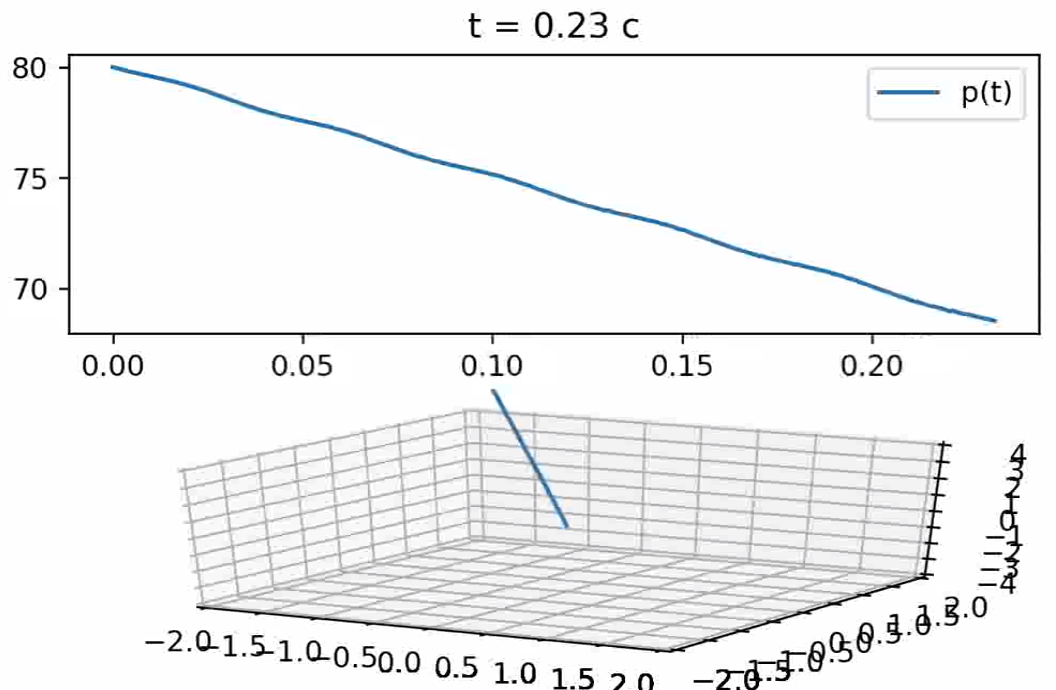
\includegraphics[width = 0.5 \textwidth]{euler_case_dissip}

\end{document} % конец документа